\documentclass[12pt,onecolumn]{article}
\usepackage{amssymb,gensymb, amsmath, amsthm,graphicx, paralist,algpseudocode,cancel,url,color,setspace}
\usepackage{fancyhdr}
\usepackage[ruled,vlined,noend]{algorithm2e}
\usepackage{sectsty}
\usepackage{fancyvrb}
\usepackage{mathrsfs}
\usepackage{multirow}
\usepackage{hhline}
\usepackage{booktabs}
\usepackage[table]{xcolor}
\usepackage{tikz}
\usepackage{amsmath}
\usepackage{graphicx}
\graphicspath{ {./graphs/} }
\usepackage{hyperref}
\hypersetup{
    colorlinks=true,
    linkcolor=cyan,
    filecolor=magenta,      
    urlcolor=blue,
}
\usepackage{enumitem}
\DeclareMathOperator{\nullspace}{null}

\newcommand{\bvec}[1]{\mathbf{#1}}
\newcommand{\R}{\mathbb{R}}
\DeclareMathOperator{\Tr}{Tr}
\sectionfont{\Large\sc}
\subsectionfont{\sc}
\usepackage[margin=1 in]{geometry}
\begin{document}
\DontPrintSemicolon
\title{Predicting MLB Games}
\author{Brian Won (bw436) and Jiacheng Wu (jw2545)}
\date{December 10, 2019}
\maketitle

\section*{Intro}
Inspired by the recent MLB postseason, our initial project goal was to predict postseason games. Due to limited sample size and the extreme difficulty of predicting playoff matchups, we changed our goal to predicting regular season games. The best team often \href{https://www.espn.com/mlb/story/_/page/playoffs16_whydontthebestteamswinitall/why-difficult-best-mlb-teams-win-all}{doesn't end up winning the World Series} and there \href{https://theathletic.com/1234635/2019/09/24/sarris-what-if-anything-predicts-a-teams-success-in-the-postseason/}{aren't really any metrics} that differentiate the top postseason teams from the rest of the pack. \vspace*{4mm}

\noindent
Firstly, playoff games feature teams that are more evenly matched than are teams of regular season games. Secondly, logistics during the playoffs are different than that of the regular season; there are more days off during October baseball. This allows teams' better pitchers to get more rest before games and be brought in more often. Teams have even resorted to using their regular season starting pitchers from the bullpen (like the 2018 Red Sox). Thirdly, the playoff format features best-of-5 and best-of-7 series. It doesn't make the most sense to look at regular season stats, which come from games against teams of all tiers, to predict the outcome of games played against a single team. It may be more sensible to look at how each hitter of a lineup has historically done against the better pitchers of the other team.

\section*{Approach}
Baseball involves a ton of data from season-level to pitch-level information. Before compiling our dataset and features of interest, we planned our approach for this problem. Off the bat (pun intended), it's practical to look at the level of talent of both teams when predicting a winner. We decided to analyze "talent" by looking at recent performance of teams leading up to a game. Our reasoning is that recent performance should capture "inherent" talent of a team, but also take into account whether a team/player has been on a cold or hot streak. Because we want an applicable look-back period for the games we predict, we looked at games played after the one-month point of a season. \vspace*{4mm}

\noindent
For hitting, we compiled team-level stats because hitters individually have limited impact on a game. Hitting in baseball is truly a team effort; it takes a string of good at-bats to score runs. It's not sustainable for an offense to rely on just one or two guys while everyone else gets out all the time. We set the look-back period for hitting stats to 10 days. \vspace*{4mm}

\noindent
For pitching, we looked at featured starting pitchers because individually they have significant impact on a game. Starting pitchers usually pitch at least 5 innings. Of course there are relief pitchers (also referred to as the bullpen), but they are tricky to incorporate into our data. Different relief pitchers are used across games depending on factors such as game situation and how well-rested pitchers are. We set the look-back period for starting pitching stats to 30 days, which equates to roughly 5 previous starts.

\section*{Good Baseball Stats}
David Grabiner, Director of Quantitative Analysis for the New York Yankees, thoroughly explains what constitutes a "good" baseball stat in this \href{http://www.seanlahman.com/baseball-archive/sabermetrics/sabermetric-manifesto/}{piece}. In short, a good baseball metric is one that measures contribution to a fundamental goal of baseball and reflects a player's own contribution as much as possible. For example, let's look at batting average (BA) and on-base percentage (OBP). BA is a traditional stat that is popular and always highlighted during game broadcasts, but it doesn't quite satisfy the first criteria. The fundamental goal of hitting in baseball is to get on base, but getting a hit isn't the only way to reach base. One can look at four balls and draw a walk, but that isn't reflected in BA. OBP is the better stat because it takes walks into account. Another example is runs batted in (RBI). Intuitively, one can say a hitter with a lot of RBIs must be good. However, this is a case of a metric not solely measuring the contribution of that hitter. If his teammates who hit before him get on base often, he'll have more RBIs thanks to more opportunities. If his teammates are fast runners, he'll have more RBIs since they can score from 2nd base on a mere single.

\section*{Definitions and Formulas}
Given the plethora of stats and their acronyms, here are their definitions and formulas:
\begin{itemize}
\item Plate appearance : PA = any time a hitter comes up to bat
\item At bat : AB = Plate appearances excluding walks, hit by pitches, sacrifice bunts, and sacrifice flies
\item On-base percentage : OBP $=\displaystyle \frac{\text{Times on base}}{\text{Plate appearances}}$
\item Slugging percentage : SLG $=\displaystyle \frac{\text{Total bases from hits}}{\text{At bats}}$
\item Strikeout : K
\item Walk : BB
\item Ground ball : GB = ball hit in play on the ground
\item Fly ball : FB = ball hit in play high in the air
\item Line drive : LD = ball hit (hard) in play in the air, but not that high
\item Starting pitcher : SP
\end{itemize}

\section*{Compiling Data}
With our approach and definition of good baseball stats in mind, we then compiled our data. For team hitting stats, we pulled individual game logs from \href{https://www.retrosheet.org/gamelogs/index.html}{Retrosheet}. For starting pitchers' stats, we used the Python package \href{https://github.com/jldbc/pybaseball}{pybaseball}. There were about 180 rows for each season containing NaN values for pitching stats because those games featured a starting pitcher making his season debut or first start after coming back from extended injury. Thus, we can't calculate rolling window stats for those pitchers. Our final dataset consists of 5581 regular season games from the 2016-2018 seasons and has the following features:
\begin{itemize}
  \item \textit{date} : date of game
  \item \textit{h\textunderscore team} : home team
  \item \textit{h\textunderscore sp\textunderscore obp} : home SP on-base percentage against
  \item \textit{h\textunderscore sp\textunderscore slg} : home SP slugging percentage against
  \item \textit{h\textunderscore sp\textunderscore gb/fb} : home SP ground ball to fly ball ratio
  \item \textit{h\textunderscore sp\textunderscore ld} : home SP line drive rate
  \item \textit{h\textunderscore sp\textunderscore k/bb} : home SP strikeout to walk ratio
  \item \textit{h\textunderscore obp} : home team on-base percentage (hitting)
  \item \textit{h\textunderscore slg} : home team slugging percentage
  \item \textit{h\textunderscore k\textunderscore rate} : home team strikeout rate
  \item \textit{h\textunderscore bb\textunderscore rate} : home team walk rate
  \item \textit{v\textunderscore team} : visiting team
  \item \textit{v\textunderscore sp\textunderscore obp} : visiting SP on-base percentage against
  \item \textit{v\textunderscore sp\textunderscore slg} : visiting SP slugging percentage against
  \item \textit{v\textunderscore sp\textunderscore gb/fb} : visiting SP ground ball to fly ball ratio
  \item \textit{v\textunderscore sp\textunderscore ld} : visiting SP line drive rate
  \item \textit{v\textunderscore sp\textunderscore k/bb} : visiting SP strikeout to walk ratio
  \item \textit{v\textunderscore obp} : visiting team on-base percentage (hitting)
  \item \textit{v\textunderscore slg} : visiting team slugging percentage
  \item \textit{v\textunderscore k\textunderscore rate} : visiting team strikeout rate
  \item \textit{v\textunderscore bb\textunderscore rate} : visiting team walk rate
  \item \textit{home\textunderscore win} : boolean indicating if home team won (variable we want to predict)
\end{itemize}

\section*{Exploratory Analysis}
Of the 5581 games, the home team won about 53.6\% of the time. It makes sense that the home team tends to win slightly more, but the difference isn't drastic to the point where we have a class imbalance issue to deal with.

\begin{center}
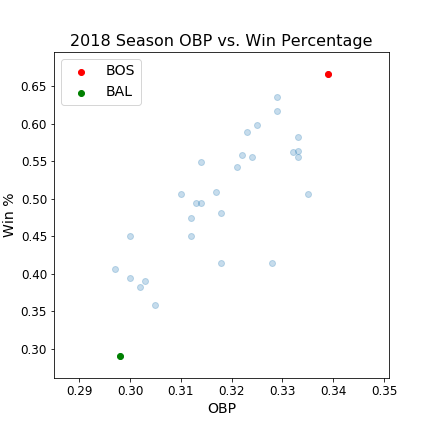
\includegraphics[scale=0.52]{obp_winp}
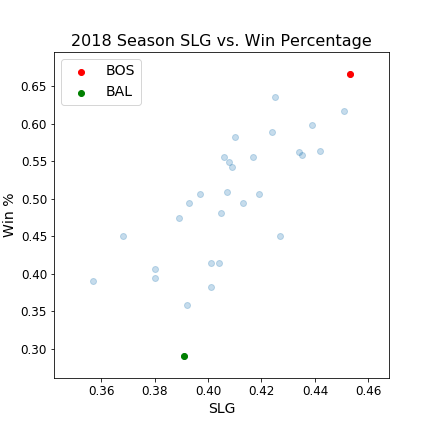
\includegraphics[scale=0.52]{slg_winp}
\end{center}

\noindent
From the plots above, we can see that winning percentage has a strong linear relationship with team on-base percentage and slugging percentage. This corroborates our notion that OBP and SLG are "good" baseball metrics.

\begin{center}
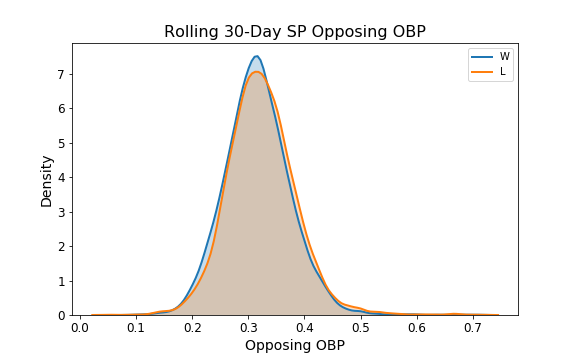
\includegraphics[scale=0.6]{sp_obp}
\end{center}

\begin{center}
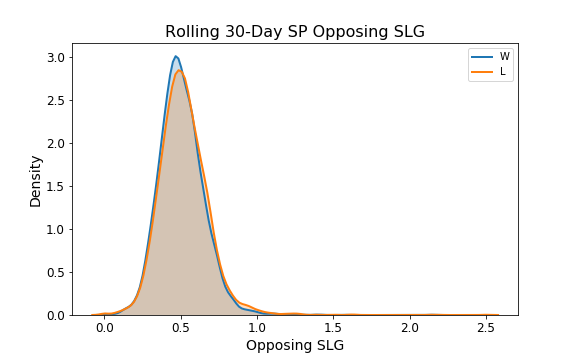
\includegraphics[scale=0.6]{sp_slg}
\end{center}

\noindent
For the two figures above, we graphed the distributions of opposing OBP and SLG for starting pitchers, dependent on if their team won the game they pitched. Interestingly, the distributions of both classes for each stat are pretty much the same. This gives us reason to believe that those SP metrics aren't very predictive for the outcome of a game.

\section*{Modeling}
Following Roger Pharr's \href{https://towardsdatascience.com/predicting-mlb-game-outcomes-with-machine-learning-594eac9484e9}{reasoning}, we believe it makes sense to judge our models against the Vegas bookkeepers. According to the 7 years of bookkeepers' data that Pharr pulled, Vegas was correct 56.7\% of the time.

\subsection*{Perceptron}
For our first model, we implemented the perceptron algorithm. Our data is most certainly not linearly separable and so we just set a cap on how many iterations the algorithm would go through. We found that randomly searching for misclassifications was more effective than searching in order. Yet, this yielded a test accuracy of 50.5\%.

\subsection*{Logistic Regression}
Next, we used logistic regression. We cross validated to search for the better regularization method between L1 and L2, and the best constant setting the strength of regularization. We correctly expected the search to result in L2 being the better method because we don't need L1 to penalize larger coefficients and produce sparser coefficients; our algorithm might as well incorporate as much data (information) that baseball can provide to make predictions. This yielded a test accuracy of 56.3\%. Pretty good.

\subsection*{Random Forest and Boosted Tree (XGBoost) Explained}
Random Forest and Boosted Trees are both variations of the Decision Tree model. A decision tree is a flowchart-like model in which each internal node represents a binary “test” on a variable. In our case, such a test can take the form of “\textit{h\textunderscore sp\textunderscore obp} $>$ 0.200”. By following and completing a series of these internal nodes, one can reach one of many terminal nodes, which in our case returns a binary prediction. \vspace*{4mm}

\noindent
The original Decision Tree model produces a decision tree by first “growing” a redundant tree in which all data points show up as terminal nodes. This redundant tree is then “pruned” by balancing between model accuracy and complexity. \vspace*{4mm}

\noindent
Random Forest and Boosted Tree are more advanced versions of the Decision Tree model. Random Forest improves upon the original implementation by growing a large number of trees (100 or 1000 is a typical number), each based on a random subset of all available variables. These trees are then aggregated by “majority vote” in our case of a classification problem. \vspace*{4mm}

\noindent
Boosted Tree improves upon the original implementation by recursively fitting new trees to the residuals of previous trees. Each subsequent tree are shrunken by a factor, typically 0.01 or 0.001. \vspace*{4mm}

\noindent
The “XGBoost” packaged used in our project provides an efficient and scalable implementation of the Boosted Tree model. It is one of the most popular data science algorithms in circulation. Introductory slides from the author of the package can be found \href{https://homes.cs.washington.edu/~tqchen/pdf/BoostedTree.pdf}{here}. \vspace*{4mm}

\noindent
After hypertuning parameters via cross validation for both methods, we obtained test case accuracies of 55.2\% for Random Forest and 54.6\% for XGBoost.

\section*{Weapon of Math Destruction}
Our project that attempts to predict the outcome of baseball games will not produce a Weapon of Math Destruction. First, baseball games do not end in ties and always produce a winner, which makes the performance of our models definitely measurable. Second, baseball is one of the most documented and most popular sports in the United States. To gain more data, we can always look further back into the past or wait for future games. Third, predictions made by our model obviously won’t affect the outcome of future games. \vspace*{4mm}

\noindent
Finally, we would like to stress that our model does not suffer from look-ahead biases. All data used to predict the outcome of a game are derived from information available prior to that game.

\section*{Fairness}
The issue of model fairness is not relevant in our case. Generally, U.S. baseball teams as competing units do not suffer from discrimination. Our methodology to predict game outcomes based on the teams’ historical performance will not put any team at an unfair advantage/disadvantage.

\section*{Conclusion}
Looking at our models and their results, we wouldn't take them to Vegas with us (yet). We believe that they can certainly be improved upon by incorporating relief pitching data and other information such as how fast pitchers throw or effects of the home team's ballpark. From one of our midterm peer reviews, there was a great suggestion of cross validating for an ideal look-back period. With beefier machines and stronger patience for long queries, that idea would be worth implementing. \vspace*{4mm}

\noindent
And as always, go Yankees.

\section*{Last Minute Update}
So we tried out the idea of taking the difference of stats between two teams. For example, instead of having \textit{h\textunderscore obp} and \textit{v\textunderscore obp}, we take the difference of the two stats to create \textit{d\textunderscore obp}. The results were much better, except for XGBoost (although we are instinctively skeptical). The test case accuracies of our models are as follows:
\begin{itemize}
\item Logistic regression : 58.2\%
\item Random Forest : 71.8\%
\item XGBoost : 53.7\%
\end{itemize}

\section*{Bibliography}
\url{https://www.espn.com/mlb/story/_/page/playoffs16_whydontthebestteamswinitall/why-difficult-best-mlb-teams-win-all} \vspace*{4mm}

\noindent
\url{https://theathletic.com/1234635/2019/09/24/sarris-what-if-anything-predicts-a-teams-success-in-the-postseason/} \vspace*{4mm}

\noindent
\url{http://www.seanlahman.com/baseball-archive/sabermetrics/sabermetric-manifesto/} \vspace*{4mm}

\noindent
\url{https://www.retrosheet.org/gamelogs/index.html} \vspace*{4mm}

\noindent
\url{https://github.com/jldbc/pybaseball} \vspace*{4mm}

\noindent
\url{https://towardsdatascience.com/predicting-mlb-game-outcomes-with-machine-learning-594eac9484e9} \vspace*{4mm}

\noindent
\url{https://homes.cs.washington.edu/~tqchen/pdf/BoostedTree.pdf}
\end{document}